\documentclass{article}
\usepackage{newtxtext,newtxmath}
\usepackage{fontsize}
\changefontsize{12pt}
\usepackage[T1]{fontenc}
\usepackage{fancyhdr}
\usepackage{graphicx}
\usepackage{fontsize}

\usepackage{booktabs}
\usepackage{adjustbox}
\usepackage{pdflscape}
\usepackage{multirow}
\usepackage[colorlinks=true,
            linkcolor=blue,
            citecolor=blue,
            urlcolor=blue]{hyperref}
\usepackage{enumitem}
\usepackage{colortbl}
\usepackage{threeparttable}
\usepackage{amsmath}
\usepackage{authblk}
\usepackage[backend = biber,
            style = apa
            ]{biblatex}

\addbibresource{referencias.bib}
\linespread{1.5}
\pagestyle{fancy}
\setlength{\parindent}{0pt}
\setlength{\parskip}{1em}
\fancyhf{}
\fancyfoot[C]{\thepage}
\fancyhfoffset{0pt}
\renewcommand{\headrulewidth}{0pt}
\renewcommand{\footrulewidth}{0pt}
\usepackage[a4paper, margin=2.54cm]{geometry}
\renewcommand{\arraystretch}{1.2}
\newcolumntype{P}[1]{>{\raggedright\arraybackslash}p{#1}}
\renewcommand{\figurename}{Figura}
\renewcommand{\tablename}{Tabla}
\usepackage{etoolbox}
\AtBeginEnvironment{table}{\linespread{1}\selectfont\renewcommand{\arraystretch}{1.0}\setlength{\parskip}{0pt}}
\AtBeginEnvironment{table*}{\linespread{1}\selectfont\renewcommand{\arraystretch}{1.0}\setlength{\parskip}{0pt}}
\AtBeginEnvironment{figure}{\linespread{1}\selectfont\renewcommand{\arraystretch}{1.0}\setlength{\parskip}{0pt}}
\AtBeginEnvironment{figure*}{\linespread{1}\selectfont\renewcommand{\arraystretch}{1.0}\setlength{\parskip}{0pt}}

\title{\textbf{Del estallido al Rechazo: cambio y estabilidad de valoraciones hacia políticas indígenas en Chile, 2016–2023}\\ [1em]
\large Trabajo de Investigación para Sociología del Estado de Bienestar (SOL3043)}

\author{Ignacio Zavala Aránguiz\\
Profesor: Luis Maldonado \\
Conteo de palabras: 4,621 en texto}
\date{2 de septiembre de 2026}

\begin{document}

\begin{figure}
    \centering
    
\includegraphics[width=0.2\linewidth]{logopuc.png}
\end{figure}
\maketitle

\newpage

\section{Introducción}

El conflicto entre el Estado y los pueblos indígenas en Chile, particularmente con el pueblo mapuche, por la propiedad, autonomía y administración de territorios, entre otros derechos de reconocimiento cultural y garantías estatales constituye una de las tensiones políticas más persistentes de la democracia post-transición \parencite{bauer2016,pairican2021}. Parte de esta tensión adquirió una visibilidad inédita durante el ciclo contencioso iniciado con el Estallido Social de 2019 y el posterior proceso constituyente 2021-2022 \parencite{piscopo2021,somma2021}, que trasladó al plano de la agenda constitucional nacional discusiones hasta entonces periféricas, poniendo en debate explícito asuntos como la plurinacionalidad y la autonomía y restitución territorial de estos pueblos, incluyéndolos en el proceso constitucional \parencite{disipavlic2024,herraz2026,montenegro2024,suarezdelucchi2024,turrachico2026}.

El reconocimiento de derechos indígenas suele entenderse como una vía de reparación de injusticias históricas \parencite{kymlicka2003}. No obstante, los Estados no siempre logran adoptar regímenes integrales de derechos indígenas, procesos que incluso pueden fracasar en su formulación e implementación \parencite{bergmann2024,turrachico2026}. El caso chileno lo ilustra claramente: pese a que la Convención Constitucional incorporó representación indígena directa poniendo en discusión diversos asuntos, la propuesta resultante fue rechazada por la ciudadanía en el plebiscito de 2022 \parencite{disipavlic2024}. Si bien las explicaciones del resultado suele anclarse a las tensiones entre actores institucionales y las convenciones de soberanía estatal, rara vez consideran la relevancia que la ciudadanía atribuye a estos temas en el tiempo. En sociedades democráticas, la sostenibilidad de una política pública depende en que su tema mantenga centralidad en la agenda ciudadana más allá de su visibilidad, lo cual plantea una pregunta previa a la del apoyo en un momento dado: si la importancia atribuida a estas políticas, una vez instalada, persiste en el tiempo o se disuelve cuando el tema pierde centralidad en el debate público. Esto resulta especialmente relevante para las políticas indígenas, sobre las cuales existe escaso conocimiento factual, baja sofisticación política y que cuentan con pocas oportunidades de ser discutidas en la agenda pública \parencite{foxworth2023,fuentes2025}.

Ahora bien, la literatura sobre estabilidad de actitudes hacia grupos étnico-raciales ofrece un punto de partida, aunque limitado para este problema. Por un lado, los estudios de panel sobre actitudes raciales y migratorias tienden a encontrar disposiciones estables una vez controlado el error de medición \parencite{kustov2021}, si bien otros muestran que incluso estas predisposiciones pueden reordenarse cuando cambia el contexto político \parencite{engelhardt2021}. Sin embargo, estos trabajos refieren a actitudes generales hacia grupos, y no a la evaluación de políticas específicas dirigidas a grupos históricamente vulnerados. Por otro lado, la investigación sobre políticas indígenas descansa mayoritariamente en encuestas transversales o diseños experimentales \parencite{alcantara2025,bergmann2024,foxworth2026,fuentes2025,pehrson2011}, o en series agregadas de encuestas repetidas \parencite{levy2022}, que permiten describir tendencias pero no distinguir si un cambio en el nivel agregado responde a una actualización persistente de las personas, a fluctuaciones transitorias o a error de medición.

Este trabajo pretende contribuir en dos sentidos. Primero, ofrece evidencia de panel sobre la importancia atribuida a políticas indígenas a lo largo de un ciclo en que estos temas alcanzaron una saliencia inédita y luego la perdieron, lo que permite observar tanto su activación como su eventual caída. Segundo, al comparar cinco políticas evaluadas por las mismas personas y con el mismo formato de pregunta, pero con distinto grado de exposición en el ciclo constituyente \parencite{disipavlic2024}, permite examinar si la estabilidad depende del tipo de política evaluada. Siguiendo a Kiley y Vaisey \parencite*{kiley2020}, entendemos por cambio persistente aquel que, una vez ocurrido en una persona, se propaga a sus respuestas posteriores, a diferencia de los desplazamientos transitorios del nivel agregado y de las fluctuaciones atribuibles a error de medición.

A partir de estos antecedentes, proponemos la siguiente pregunta de investigación: \textbf{¿En qué medida las valoraciones de distintas políticas indígenas muestran patrones de cambio persistente o estabilidad durante 2016-2023 en Chile, y cómo varía este patrón según el tipo de política evaluada?} Para responderla, empleamos cuatro olas del \textit{Estudio Longitudinal de Relaciones Interculturales} (ELRI; $N=1{,}589$) y comparamos modelos de disposiciones estables, de actualización activa y quasi-simplex para cinco políticas. 

\section{Antecedentes teóricos}

\subsection{Modelos de cambio y estabilidad de creencias}

En el marco de la literatura sobre estabilidad y cambio de creencias, Kiley y Vaisey \parencite*{kiley2020} formalizan dos modelos de cambio individual. El primero es el \textit{modelo de disposiciones estables} (SDM), que sostiene que las personas reportan sus actitudes desde una creencia basal, de modo que las fluctuaciones observadas entre olas son en gran medida error de medición o desviaciones transitorias que no se arrastran a mediciones posteriores. El \textit{modelo de actualización activa} (AUM), en cambio, postula que las personas revisan sus creencias ante información nueva en su entorno, y que ese cambio se propaga hacia sus respuestas futuras en dicho asunto. La virtud de esta reformulación es que convierte una discusión históricamente teórica en dos especificaciones estructurales comparables empíricamente: en vez de preguntar, como la tradición en opinión pública, si las personas poseen o no creencias consistentes \parencite{achen1975,ansolabehere2008,converse1964}, examinan qué fuentes explican el cambio temporal de las respuestas \parencite{vaisey2021}.

En el dominio de las actitudes raciales-étnicas, la evidencia favorece mayoritariamente al SDM. Kiley y Vaisey \parencite*{kiley2020}, al analizar 183 ítems de la \textit{General Social Survey}, encuentran que la mayoría de los ítems sobre raza no muestra evidencia de actualización, lo que sugiere visiones asentadas antes de la adultez, resultado que Vaisey y Kiley \parencite*{vaisey2021} refuerzan con más de 500 ítems. Kustov et al. \parencite*{kustov2021}, por su parte, muestran en nueve paneles que las actitudes hacia la inmigración resisten incluso shocks económicos y políticos importantes. No obstante, esta estabilidad no es uniforme. Los mismos Kiley y Vaisey \parencite*{kiley2020} advierten que varios ítems raciales son tan inconsistentes entre olas que difícilmente pueden calificarse como asentados o en actualización, y que las preguntas sobre políticas específicas, que tratan como creencias \textit{periféricas}, muestran mayor evidencia de actualización y menor consistencia. Engelhardt \parencite*{engelhardt2021}, a su vez, muestra que las actitudes raciales de votantes blancos estadounidenses se alinean con su identificación partidaria, influencia que se intensifica cuando cambia el contexto político, mientras que Levy y McAllister \parencite*{levy2022} documentan una liberalización sostenida de la opinión pública australiana sobre temas indígenas en tres décadas. Así, la evidencia disponible refiere a actitudes generales hacia grupos o a tendencias agregadas, y no resuelve si la importancia atribuida a políticas específicas se comporta como una predisposición estable o como una creencia periférica sensible al contexto.

Una dificultad de esta comparación es que el SDM y el AUM se estiman sobre respuestas observadas, de modo que el error de medición puede atenuar la persistencia estimada del AUM y favorecer artificialmente al SDM. La evidencia a favor de la estabilidad aparece, de hecho, sistemáticamente cuando el error se controla de forma explícita, ya sea promediando múltiples ítems de un mismo dominio \parencite{ansolabehere2008} o mediante el \textit{modelo quasi-simplex} (QSM) de Wiley y Wiley \parencite*{wiley1970}, reforzado por Achen \parencite*{achen1975}, que separa el \textit{true score} individual del error mediante una cadena autorregresiva de al menos tres olas. Con este modelo, Prior \parencite*{prior2010} encuentra que el interés político es una disposición excepcionalmente estable en paneles de varios países, y Kustov et al. \parencite*{kustov2021} sostienen su conclusión sobre inmigración. El QSM cumple, por tanto, un doble rol en esta discusión. Por una parte, dado que modela un proceso en que el \textit{true score} de cada ola depende del anterior, puede leerse como una versión del AUM corregida por error de medición \parencite{kiley2020}: si la desventaja del AUM se debiera solo a atenuación, el QSM debiera ajustarse claramente mejor que el SDM. Por otra, al estimar un coeficiente de estabilidad para cada transición, permite localizar en qué períodos se concentra el cambio.

La literatura ofrece, sin embargo, expectativas encontradas respecto del rol de la saliencia. Sears \parencite*{sears1983} sostiene que la estabilidad de una actitud es función de su objeto, y que es mayor cuando este es concreto, manifiesto y saliente, argumento que Prior \parencite*{prior2010} retoma para explicar la persistencia del interés político. Kiley y Vaisey \parencite*{kiley2020}, en cambio, encuentran que el cambio persistente es más probable en temas públicos de alto perfil, como ocurrió con los derechos de las personas homosexuales, y sugieren que la mayoría de los temas simplemente no alcanza la saliencia necesaria para modificar opiniones. Por último, en línea con las consideraciones accesibles de Zaller y Feldman \parencite*{zaller1992}, un evento de alta visibilidad puede incorporar consideraciones nuevas que vuelven a ser muestreadas en encuestas posteriores. En otras palabras, la saliencia podría anclar las valoraciones como desplazarlas, lo que hace relevante examinar contextos en que la exposición pública de distintas políticas varía de manera marcada.


\subsection{El caso chileno: conflicto indígena y el proceso constituyente post-estallido}

El conflicto entre el Estado chileno y los pueblos indígenas por la propiedad y administración de territorios, especialmente en la macrozona sur, antecede ampliamente al período examinado, desde la promulgación de la Ley Indígena de 1993 hasta la escalada de represión y violencia en la Araucanía \parencite{montenegro2024,pairican2021}. Su carácter continuo, aunque de visibilidad nacional variable, explica que su reactivación durante el estallido social de 2019 represente la elevación de una tensión preexistente a un lugar inédito en la agenda pública \parencite{piscopo2021,somma2021}. El proceso constituyente acordado en respuesta al estallido puso en debate explícito, junto con temas sobre derechos básicos de salud, pensiones y educación, asuntos como la plurinacionalidad, la autonomía territorial y la restitución de tierras, e incorporó escaños reservados para los pueblos indígenas en la Convención \parencite{bauer2018,disipavlic2024,herraz2026,turrachico2026}. De este modo, la administración autónoma de territorios, la restitución de tierras y los escaños reservados dejaron de ser contenidos sectoriales o regionales para integrar la agenda de reforma constitucional nacional. Otras políticas orientadas a la calidad de vida de la población indígena, como mejorar su educación y empleo, permanecieron en cambio como política social secundaria, sin un lugar equivalente en el debate sobre el rediseño del Estado \parencite{suarezdelucchi2024} y más bien como demandas transversales a toda la población \parencite{somma2021}.

El Rechazo de la propuesta en el plebiscito de septiembre de 2022, seguido de un segundo proceso con una participación indígena más acotada \parencite{turrachico2026}, constituye un segundo quiebre. Esta secuencia permite distinguir tres fases que coinciden con las transiciones del panel: pre-estallido (2016-2018), estallido y proceso constituyente (2018-2021) y post-Rechazo (2021-2023). El último tramo resulta particularmente informativo, en tanto permite observar si la importancia atribuida a las políticas instaladas durante el proceso constituyente se mantiene una vez que el tema indígena pierde centralidad, o si retrocede hacia sus niveles previos \parencite{kiley2020}. Esta secuencia de eventos ofrece una oportunidad casi natural para testear si los cambios observados en la relevancia atribuida a políticas indígenas fueron persistentes o transitorios, y si ese patrón depende del contenido en el debate constitucional. A partir de esta discusión, proponemos las siguientes hipótesis:

\begin{quote}
\textbf{H1:} \textit{La importancia atribuida a las políticas discutidas en la Convención (autonomía territorial, escaños reservados y restitución de tierras) se ajustará mejor a un modelo de actualización activa (AUM), mientras que la atribuida a las políticas socioeconómicas (educación y empleo) se ajustará mejor a un modelo de disposiciones estables (SDM).}
\end{quote}

Las primeras corresponden a demandas de reconocimiento y rediseño institucional cualitativamente distintas de la política social convencional \parencite{bauer2016}, que durante el ciclo constituyente alcanzaron una saliencia pública que Kiley y Vaisey \parencite*{kiley2020} asocian a procesos de actualización, en tanto un evento de alta visibilidad puede incorporar consideraciones nuevas que vuelven a ser muestreadas en encuestas posteriores \parencite{zaller1992}. Las segundas, en cambio, permanecieron como política social secundaria, por lo que cabe esperar en ellas el predominio de disposiciones estables que la literatura documenta para actitudes raciales y migratorias \parencite{kustov2021,vaisey2021}.

\begin{quote}
\textbf{H2:} \textit{En las políticas discutidas en la Convención, la estabilidad de las valoraciones será menor en la transición 2018-2021 que en las demás transiciones, y su nivel promedio se desplazará en 2021; en las políticas socioeconómicas, tanto la estabilidad como el nivel se mantendrán constantes entre transiciones.}
\end{quote}

Si, como sostienen Kiley y Vaisey \parencite*{kiley2020}, la saliencia pública es la condición que permite que las opiniones se desplacen, ese desplazamiento debiera expresarse en la transición que contiene el estallido y el proceso constituyente, mientras que las políticas que no ocuparon un lugar equivalente en ese debate no tendrían motivo para variar \parencite{suarezdelucchi2024}. El QSM permite evaluar esta expectativa al estimar la estabilidad y el nivel de cada ola libres de error de medición.

\section{Metodología}

\subsection{Datos}

Emplearemos cuatro olas del \textit{Estudio Longitudinal de Relaciones Interculturales} (ELRI), realizado por el Centro de Estudios Interculturales e Indígenas [CIIR] de Chile, un panel fijo repetido que entrevista a miembros de la población indígena y no indígena de Chile cada 18-24 meses en tres macrozonas del país (Norte, Centro y Sur), levantado entre los años 2016 y 2023. El diseño emplea un muestreo de población atípica que sobrerrepresenta a la población indígena, complementado con un esquema de ``muestras espejo'': dentro de las mismas manzanas o entidades rurales se seleccionan de forma probabilística tanto personas autoidentificadas con pueblos originarios como personas no indígenas, controlando así por proximidad espacial entre ambos grupos. El tamaño muestral disponible por ola es de 3.617 (2016), 2.879 (2018), 1.847 (2021) y 1.680 (2023) personas entrevistadas en al menos tres de las cuatro mediciones, con la mayor pérdida de casos ocurriendo entre la Ola 2 y la Ola 3, coincidente con el cambio forzado de modalidad presencial a telefónica durante la pandemia de COVID-19. Este informe emplea un panel balanceado más estricto, restringido a personas con información válida en las cuatro olas ($N=1{,}589$)\footnote{El manual metodológico del ELRI documenta una atrición diferencial: la permanencia hasta 2023 fue menor entre hombres (38,5\% frente a 50,8\% en mujeres), en la muestra no mapuche (42,3\%) y, sobre todo, entre quienes ingresaron al estudio con 18 a 34 años (23,1\%). El manual ofrece ponderadores longitudinales construidos por probabilidad inversa, que el análisis principal no incorpora al no hallarse en la base de datos pública.}.



\subsection{Variables y estrategia analítica}

Nuestra variable dependiente consta de cinco ítems del módulo de Políticas Públicas, referidos a la importancia atribuida a diversas políticas indígenas, aplicados en las cuatro olas: \textit{``Existe una serie de políticas que se han discutido para abordar el tema indígena. Según usted, ¿cuán importante es...?''}, siendo evaluadas ``Políticas de generación de empleo'', ``Que puedan administrar autónomamente sus territorios'', ``Mejorar su educación'', ``Restituirles o devolverles sus tierras'' y ``Establecer asientos especiales en el congreso''. Todas son evaluadas mediante una escala de intensidad de 5 puntos (1 = Muy poco, 5 = Mucho). Nótese que estos ítems consideran tanto políticas de integración socioeconómica (empleo y educación) como políticas de reconocimiento cultural y territorial (autonomía, restitución de tierras y escaños reservados), lo que permite contrastar si la relevancia atribuida a cada tipo de política se comporta de forma distinta en el tiempo. Cabe notar que estos ítems miden la importancia atribuida a cada política y no el apoyo a ella.

La estrategia analítica tiene dos etapas, correspondientes a cada hipótesis. Para H1, siguiendo a Vaisey y Kiley \parencite*{vaisey2021}, estimamos para cada ítem cuatro modelos expresados como restricciones de la Ecuación~\ref{eq:general},

\begin{equation}
y_{it} = \alpha_t + \rho_t\, y_{i,t-1} + U_i + \varepsilon_{it}
\label{eq:general}
\end{equation}

donde $y_{it}$ es la importancia atribuida por la persona $i$ a una política en la ola $t$; $\alpha_t$, un intercepto propio de cada ola que capta shocks agregados que desplazan a todas las personas por igual; $\rho_t$, la persistencia de la respuesta entre olas consecutivas; $U_i$, una disposición individual fija; y $\varepsilon_{it}$, un componente transitorio cuya varianza puede diferir entre olas. Los modelos SDM fijan $\rho_t = 0$ y estiman la varianza de $U_i$, y se distinguen en si el intercepto es libre por ola o constante; los modelos AUM fijan $U_i = 0$ y se distinguen en si el intercepto y la persistencia son constantes o libres por ola (Tabla~\ref{tab:especificaciones}). Esto resulta en 20 modelos (4 especificaciones $\times$ 5 ítems), estimados en \texttt{lavaan} con máxima verosimilitud robusta (MLR). Para H2, y para controlar la atenuación por error de medición que afecta a los modelos anteriores, estimamos además un QSM por ítem \parencite{prior2010,wiley1970}, que separa una ecuación de medición de una estructural:

\begin{equation}
y_{it} = \eta_{it} + \varepsilon_{it}, \qquad \eta_{it} = \alpha_t + \beta_{t,t-1}\,\eta_{i,t-1} + \zeta_{it}
\label{eq:qsm}
\end{equation}

donde $\eta_{it}$ es el \textit{true score}, $\beta_{t,t-1}$ la estabilidad entre olas consecutivas libre de error de medición, y $\zeta_{it}$ el cambio nuevo que ingresa en cada ola. Con un solo indicador por ola, la identificación exige fijar la carga en 1 y suponer una varianza de error igual en las cuatro olas, lo que deja 2 grados de libertad\footnote{En generación de empleo, la varianza de $\zeta$ en 2018 resultó levemente negativa ($\approx -0{,}001$), un caso Heywood, por lo que se fijó en cero (3 grados de libertad). Los coeficientes de estabilidad prácticamente no cambian (.72, .71 y .34), y la correlación 2016-2018 igual a 1 debe leerse como un valor de frontera, no como estabilidad perfecta.}. 


\begin{table}[ht!]
\caption{Especificaciones de los modelos SDM y AUM}
\label{tab:especificaciones}
\centering
\resizebox{0.8\textwidth}{!}{
\begin{tabular}{llcccc}
\toprule
 & & \multicolumn{3}{c}{\textbf{Restricciones}} & \\
\cmidrule(lr){3-5}
\textbf{Modelo} & \textbf{Versión} & $\boldsymbol{U_i}$ & $\boldsymbol{\rho_t}$ & $\boldsymbol{\alpha_t}$ & \textbf{gl} \\
\midrule
SDM & Libre     & Varianza libre & 0             & Libre por ola & 5 \\
    & Puro      & Varianza libre & 0             & Constante     & 8 \\
\midrule
AUM & Constante & 0              & Constante     & Constante     & 7 \\
    & Libre     & 0              & Libre por ola & Libre por ola & 3 \\
\bottomrule
\multicolumn{6}{l}{\rule{0pt}{1em}\footnotesize\textbf{Nota:} Restricciones sobre la Ecuación~\ref{eq:general}. En todos los modelos la varianza de $\varepsilon_{it}$ es libre por ola.} \\
\multicolumn{6}{l}{\footnotesize gl: grados de libertad.} \\
\end{tabular}
}
\end{table}


Puesto que $\beta_{t,t-1}$ es una pendiente que depende también de cómo cambia la dispersión entre olas, reportamos además la correlación entre \textit{true scores} consecutivos; el nivel promedio de cada ola, $\mu_t = \alpha_t + \beta_{t,t-1}\,\mu_{t-1}$, y sus diferencias entre olas. Los modelos se comparan mediante el BIC como criterio principal, complementado con CFI, RMSEA y SRMR, y serán estimados con el paquete de \texttt{R lavaan}  \parencite{kline2023}. 


\newpage

\section{Resultados}

\begin{figure}[ht!]
\caption{Importancia atribuida a políticas indígenas por ola}
\label{fig:medias}
\centering
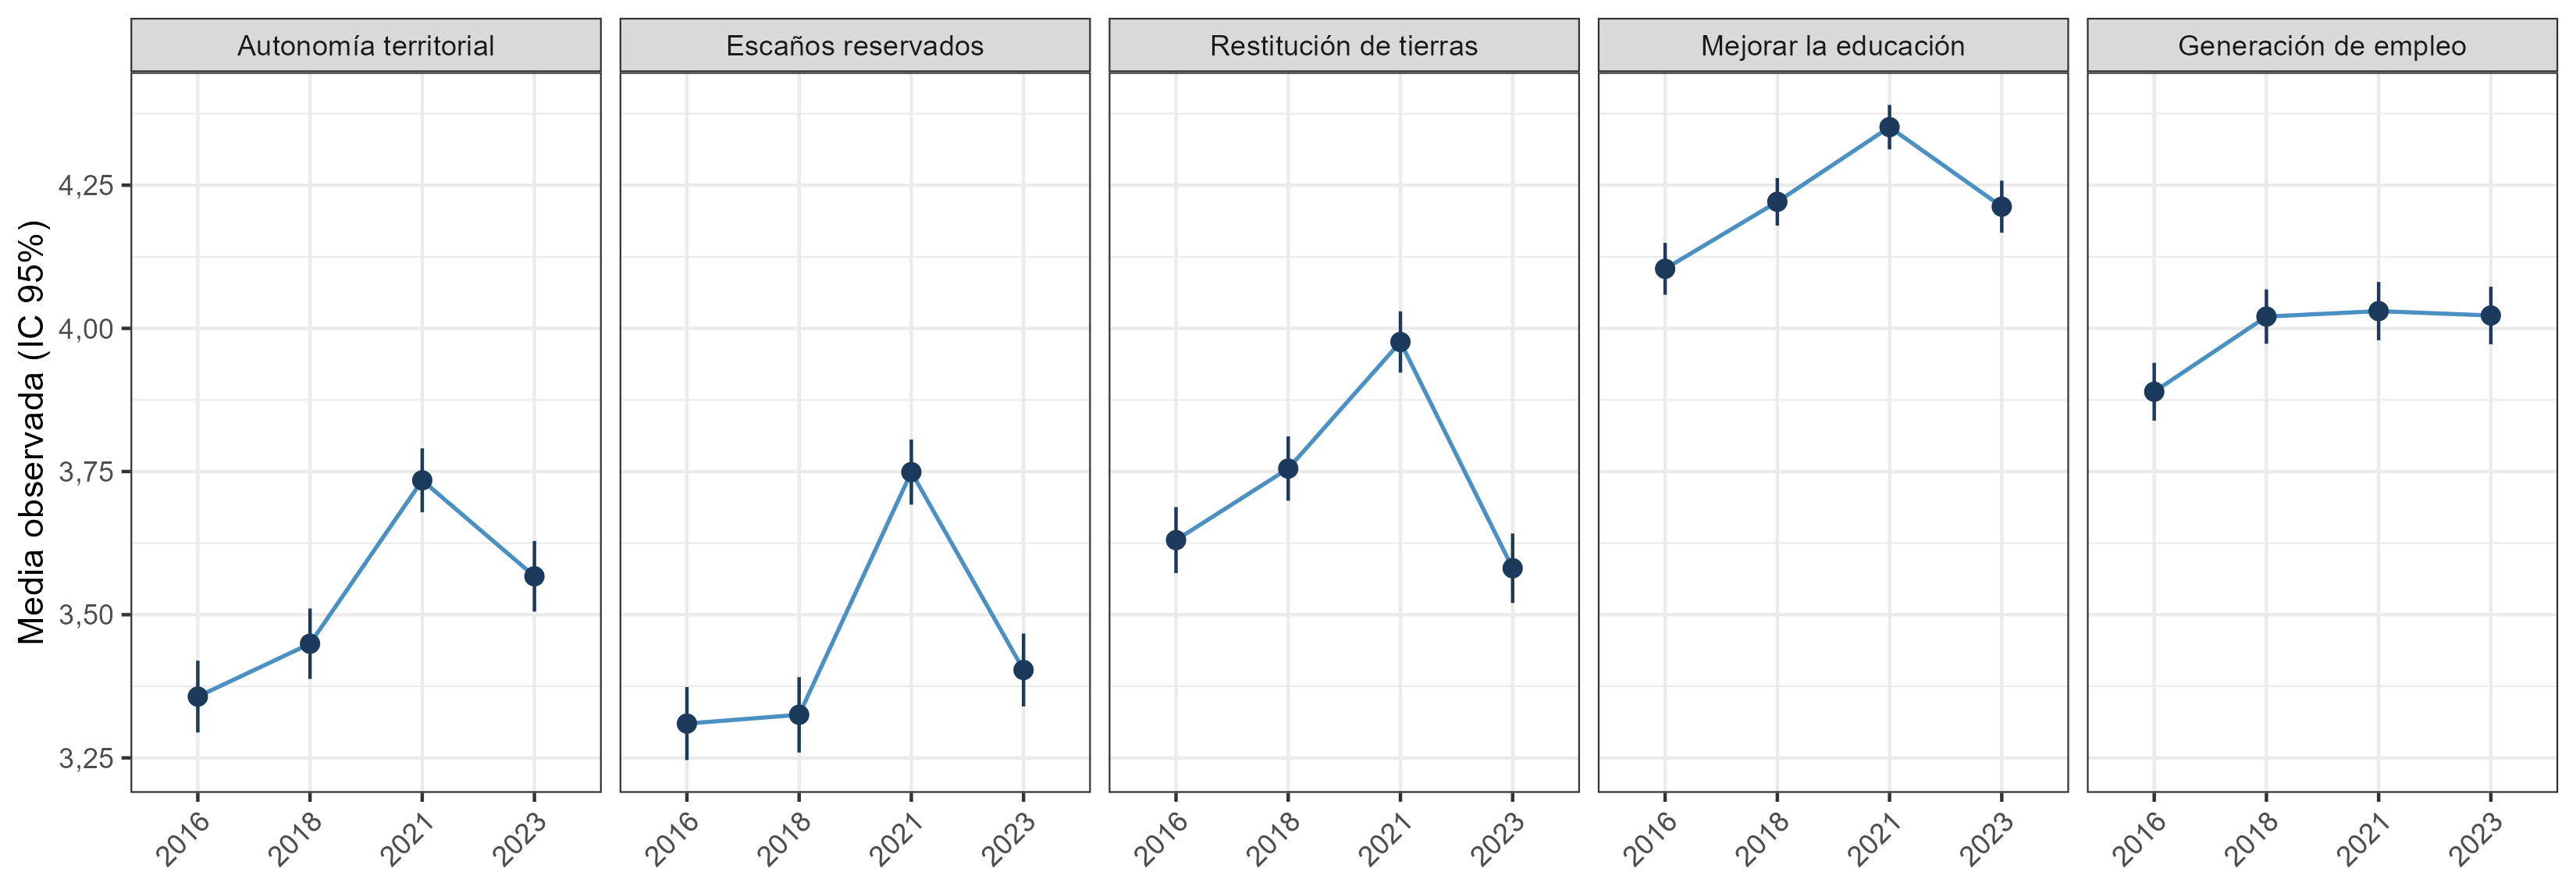
\includegraphics[width=\textwidth]{fig_medias_por_ola.png}
\begin{minipage}{\textwidth}
\footnotesize\textbf{Nota:} Medias observadas e intervalos de confianza al 95\% (1 = Muy poco, 5 = Mucho). Panel balanceado, \textit{N} = 1,589. 
\end{minipage}
\end{figure}

La Figura~\ref{fig:medias} presenta las medias observadas de la importancia atribuida a cada política por ola, junto con su intervalo de confianza al 95\%. Casi todas las políticas suben levemente entre 2016 y 2018, antes del estallido, por lo que tomamos 2018 como el nivel de referencia previo al ciclo contencioso. Desde ahí, cuatro de las cinco políticas alcanzan su nivel más alto en 2021 y retroceden en 2023, aunque con magnitudes distintas según el tipo de política. Los desplazamientos más marcados corresponden a las políticas discutidas en la Convención: escaños reservados pasa de 3,32 en 2018 a 3,75 en 2021 y vuelve a 3,40 en 2023, restitución de tierras termina bajo su nivel de 2018 (3,58 frente a 3,75) y autonomía territorial queda sobre él (3,57 frente a 3,45). Las políticas socioeconómicas, en cambio, parten de niveles más altos y varían menos: educación repite el patrón con menor amplitud, y empleo permanece en torno a 4,02 desde 2018. Dicho esto, estas medias no permiten distinguir si estos desplazamientos observados reflejan cambios en las disposiciones individuales, shocks agregados transitorios o error de medición, distinción que abordan los modelos de la sección siguiente.

La Tabla~\ref{tab:ajuste_completo} presenta los indicadores de ajuste de los cinco modelos estimados para cada política. El SDM con interceptos libres obtiene el menor BIC en cuatro de las cinco políticas, incluidas autonomía territorial y restitución de tierras, mientras que ninguna versión del AUM resulta preferida en las políticas discutidas en la Convención. Liberar el intercepto por ola mejora sustantivamente el ajuste respecto del SDM puro, con reducciones del BIC entre 49 y 143 puntos, lo que indica que las disposiciones individuales coexisten con shocks agregados propios 

\begin{table}[ht!]
\caption{Ajuste completo de los modelos por política}
\label{tab:ajuste_completo}
\centering
\resizebox{1.0\textwidth}{!}{
\begin{tabular}{llcccccc}
\toprule
\textbf{Política} & \textbf{Modelo} & \textbf{gl} & \textbf{BIC} & \textbf{CFI} & \textbf{TLI} & \textbf{RMSEA} & \textbf{SRMR} \\
\midrule
Autonomía territorial & SDM libre     & 5 & \textbf{19.589} & 0{,}865 & 0{,}838 & 0{,}058 & 0{,}037 \\
                      & SDM puro      & 8 & 19.670 & 0{,}351 & 0{,}513 & 0{,}100 & 0{,}075 \\
                      & AUM constante & 7 & 19.641 & 0{,}532 & 0{,}599 & 0{,}091 & 0{,}067 \\
                      & AUM libre     & 3 & 19.612 & 0{,}812 & 0{,}623 & 0{,}088 & 0{,}046 \\
                      & QSM           & 2 & 19.590 & 0{,}960 & 0{,}880 & 0{,}050 & 0{,}020 \\
\midrule
Escaños reservados    & SDM libre     & 5 & 20.004 & 0{,}875 & 0{,}850 & 0{,}066 & 0{,}042 \\
                      & SDM puro      & 8 & 20.148 & 0{,}283 & 0{,}462 & 0{,}124 & 0{,}094 \\
                      & AUM constante & 7 & 20.152 & 0{,}289 & 0{,}390 & 0{,}132 & 0{,}093 \\
                      & AUM libre     & 3 & 20.026 & 0{,}841 & 0{,}682 & 0{,}096 & 0{,}051 \\
                      & QSM           & 2 & \textbf{19.989} & 1{,}000 & 1{,}000 & 0{,}000 & 0{,}009 \\
\midrule
Restitución de tierras & SDM libre    & 5 & \textbf{18.931} & 0{,}985 & 0{,}982 & 0{,}027 & 0{,}022 \\
                      & SDM puro      & 8 & 19.055 & 0{,}618 & 0{,}714 & 0{,}108 & 0{,}077 \\
                      & AUM constante & 7 & 19.126 & 0{,}451 & 0{,}530 & 0{,}138 & 0{,}099 \\
                      & AUM libre     & 3 & 19.032 & 0{,}758 & 0{,}515 & 0{,}140 & 0{,}071 \\
                      & QSM           & 2 & 18.948 & 0{,}992 & 0{,}975 & 0{,}032 & 0{,}013 \\
\midrule
Mejorar la educación  & SDM libre     & 5 & \textbf{15.939} & 0{,}905 & 0{,}886 & 0{,}020 & 0{,}018 \\
                      & SDM puro      & 8 & 15.988 & 0{,}000 & $-$0{,}586 & 0{,}075 & 0{,}059 \\
                      & AUM constante & 7 & 15.953 & 0{,}128 & 0{,}253 & 0{,}051 & 0{,}040 \\
                      & AUM libre     & 3 & 15.952 & 0{,}910 & 0{,}819 & 0{,}025 & 0{,}018 \\
                      & QSM           & 2 & 15.956 & 0{,}965 & 0{,}895 & 0{,}019 & 0{,}012 \\
\midrule
Generación de empleo  & SDM libre     & 5 & 17.667 & 0{,}752 & 0{,}702 & 0{,}049 & 0{,}034 \\
                      & SDM puro      & 8 & 17.667 & 0{,}500 & 0{,}625 & 0{,}055 & 0{,}046 \\
                      & AUM constante & 7 & \textbf{17.650} & 0{,}800 & 0{,}829 & 0{,}037 & 0{,}033 \\
                      & AUM libre     & 3 & 17.674 & 0{,}823 & 0{,}646 & 0{,}054 & 0{,}029 \\
                      & QSM           & 3 & 17.658 & 1{,}000 & 1{,}058 & 0{,}000 & 0{,}006 \\
\bottomrule
\multicolumn{8}{l}{\rule{0pt}{1em}\footnotesize\textbf{Nota:} En negrita, el menor BIC de cada política. SDM y AUM con varianza de error libre por ola; QSM con varianza de error} \\
\multicolumn{8}{l}{\footnotesize igual entre olas. En empleo, el QSM fija en 0 la varianza de $\zeta_{2018}$. Estimación MLR con FIML. \textit{N} = 1,589.} \\
\end{tabular}
}
\end{table}

de cada ola. El QSM, que corrige la persistencia controlando por error de medición, resulta preferido en escaños reservados (19.989 frente a 20.004 del SDM libre) y prácticamente empata con el SDM libre en autonomía territorial (19.590 frente a 19.589). Además, presenta el mejor ajuste absoluto en todas las políticas (CFI entre 0,96 y 1,00), mientras que el del SDM libre es moderado en autonomía y escaños (CFI de 0,87 y 0,88), de modo que la ventaja del SDM en el BIC descansa en buena medida en su mayor parsimonia. En empleo, por último, el AUM constante obtiene el menor BIC, aunque con una ventaja acotada y un ajuste absoluto débil (CFI = 0,80). En consecuencia, H1 no se sostiene en las políticas de la Convención, con la salvedad de escaños reservados, y para las políticas  socioeconómicas se cumple solo en educación.

\begin{table}[ht!]
\caption{Estabilidad y nivel de la importancia atribuida según el QSM}
\label{tab:qsm}
\centering
\resizebox{\textwidth}{!}{
\begin{tabular}{lccccc}
\toprule
 & \multicolumn{3}{c}{\textbf{Discutidas en la Convención}} & \multicolumn{2}{c}{\textbf{Socioeconómicas}} \\
\cmidrule(lr){2-4}\cmidrule(lr){5-6}
 & \textbf{Autonomía} & \textbf{Escaños} & \textbf{Restitución} & \textbf{Educación} & \textbf{Empleo} \\
\midrule
\multicolumn{6}{l}{\textit{Panel A. Estabilidad entre olas}} \\[2pt]
$\beta_{2016\text{-}18}$ & 0{,}806 (0{,}131) & 0{,}917 (0{,}125) & 0{,}758 (0{,}093) & 0{,}302 (0{,}130) & 0{,}720 (0{,}121) \\
$\beta_{2018\text{-}21}$ & 0{,}465 (0{,}089) & 0{,}430 (0{,}056) & 0{,}784 (0{,}090) & 0{,}261 (0{,}130) & 0{,}711 (0{,}179) \\
$\beta_{2021\text{-}23}$ & 0{,}854 (0{,}178) & 0{,}857 (0{,}140) & 0{,}851 (0{,}092) & 0{,}922 (0{,}771) & 0{,}337 (0{,}112) \\
$r_{2016\text{-}18}$ & 0{,}877 & 0{,}847 & 0{,}840 & 0{,}417 & 1{,}000$^{a}$ \\
$r_{2018\text{-}21}$ & 0{,}615 & 0{,}673 & 0{,}843 & 0{,}392 & 0{,}480 \\
$r_{2021\text{-}23}$ & 0{,}602 & 0{,}578 & 0{,}620 & 0{,}437 & 0{,}357 \\[4pt]
\multicolumn{6}{l}{\textit{Panel B. Nivel promedio}} \\[2pt]
$\mu_{2016}$ & 3{,}354 (0{,}032) & 3{,}309 (0{,}032) & 3{,}625 (0{,}029) & 4{,}104 (0{,}023) & 3{,}889 (0{,}026) \\
$\mu_{2018}$ & 3{,}447 (0{,}031) & 3{,}321 (0{,}034) & 3{,}747 (0{,}029) & 4{,}221 (0{,}021) & 4{,}018 (0{,}024) \\
$\mu_{2021}$ & 3{,}734 (0{,}028) & 3{,}747 (0{,}029) & 3{,}972 (0{,}027) & 4{,}351 (0{,}020) & 4{,}028 (0{,}026) \\
$\mu_{2023}$ & 3{,}565 (0{,}031) & 3{,}402 (0{,}032) & 3{,}582 (0{,}031) & 4{,}212 (0{,}023) & 4{,}023 (0{,}026) \\[4pt]
\multicolumn{6}{l}{\textit{Panel C. Diferencias de nivel}} \\[2pt]
$\mu_{2021}-\mu_{2018}$ & 0{,}287* (0{,}039) & 0{,}425* (0{,}040) & 0{,}225* (0{,}034) & 0{,}130* (0{,}028) & 0{,}010 (0{,}034) \\
$\mu_{2023}-\mu_{2021}$ & $-$0{,}168* (0{,}039) & $-$0{,}344* (0{,}040) & $-$0{,}391* (0{,}036) & $-$0{,}139* (0{,}029) & $-$0{,}006 (0{,}035) \\
$\mu_{2023}-\mu_{2018}$ & 0{,}118* (0{,}043) & 0{,}081 (0{,}044) & $-$0{,}166* (0{,}038) & $-$0{,}009 (0{,}031) & 0{,}004 (0{,}035) \\
$\mu_{2023}-\mu_{2016}$ & 0{,}211* (0{,}042) & 0{,}093* (0{,}043) & $-$0{,}043 (0{,}039) & 0{,}108* (0{,}032) & 0{,}133* (0{,}036) \\
\bottomrule
\multicolumn{6}{l}{\rule{0pt}{1em}\footnotesize\textbf{Nota:} Errores estándar entre paréntesis. $\beta$: coeficiente de estabilidad no estandarizado; $r$: correlación entre \textit{true scores} consecutivos,} \\
\multicolumn{6}{l}{\footnotesize $r_{t,t-1} = \beta_{t,t-1}\sqrt{V(\eta_{t-1})/V(\eta_t)}$. * $|z| > 1{,}96$. $^{a}$ Valor de frontera, producto de fijar en 0 la varianza de $\zeta_{2018}$. \textit{N} = 1.589.} 
\end{tabular}
}
\end{table}

La Tabla~\ref{tab:qsm} presenta, a partir del QSM, la correlación entre los \textit{true scores} de olas consecutivas, que indica cuánto se mantiene el orden relativo de las personas una vez controlado el error de medición, junto con el nivel promedio de cada ola y sus diferencias. En las políticas discutidas en la Convención, las correlaciones son altas entre 2016 y 2018 (entre 0,84 y 0,88), caen entre 2018 y 2021 en autonomía territorial y escaños reservados (0,61 y 0,67) y se mantienen entre 2021 y 2023 (en torno a 0,60), mientras que restitución de tierras mantiene su estabilidad hasta 2021 (0,84) y solo la reduce en la última transición (0,62). En el período constituyente (2018-2021), además, el nivel promedio de las tres políticas sube entre 0,22 y 0,43 puntos, para retroceder en 2023: escaños vuelve a su nivel de 2018, autonomía queda 0,12 puntos sobre él y restitución, 0,17 puntos bajo él. Las políticas socioeconómicas, en cambio, presentan correlaciones bajas, inferiores a 0,50 desde 2018 y sin un quiebre en el período constituyente. En cuanto al nivel, educación sube y retrocede con menor amplitud (0,13 y $-$0,14 puntos), mientras que empleo no muestra variación notable desde 2018. En suma, H2 se sostiene en autonomía territorial y escaños reservados; en restitución de tierras el nivel se desplaza sin una caída de la estabilidad en el período constituyente, y entre las socioeconómicas, educación muestra un desplazamiento de nivel menor, aunque significativo.


\newpage


\section{Discusión y conclusiones}

Este trabajo abordó en qué medida la importancia atribuida a distintas políticas indígenas muestra cambio persistente o estabilidad durante el ciclo contencioso chileno. Los resultados sugieren cambios principalmente transitorios, cuya intensidad fue atingente al tipo de política: H1 no se sostiene, salvo en escaños reservados, y H2 se cumple en autonomía territorial y escaños reservados, y de forma parcial en restitución de tierras y educación.

Bajo la lectura del SDM, el alza de 2021 constituye una desviación temporal respecto de las disposiciones previas al estallido: los interceptos libres por ola capturan precisamente shocks que desplazan a la mayoría en una misma dirección sin alterar la creencia basal de cada persona \parencite{kiley2020}. El retorno de escaños y, en menor medida, de autonomía hacia sus niveles preestallido, así como el de restitución a su nivel de 2016, sugiere así una activación latente y momentánea donde la centralidad pública de estos temas volvió accesibles ciertas consideraciones \parencite{zaller1992} que dejaron de emerger cuando salieron de la discusión. El retroceso puede ser, además, una posible expresión de un agotamiento temático documentado: fracasada la propuesta que llevó estas demandas al plano constitucional, el segundo proceso las retiró de la discusión, sin escaños reservados y con un consejo dominado por sectores que reemplazaron la plurinacionalidad por una noción de nación única \parencite{turrachico2026,herraz2026}, en un contexto de baja valoración ciudadana del propio proceso \parencite{lazcano-pena2025,}. Esta interpretación, no obstante, no es observable en nuestros datos, y debe tomarse con mesura.

Las características de los ítems ayudan a comprender por qué este patrón se concentra en las políticas de la Convención. Estos miden importancia y no apoyo, por lo que son sensibles a la agenda deliberativa: cuando un tema ocupa el centro del debate, su importancia puede aumentar incluso entre quienes se oponen a la política. A la vez, refieren a objetos concretos, disputados y de significado relativamente constante, lo que, siguiendo a Sears \parencite*{sears1983}, favorece posiciones estables entre personas, como muestran sus altas correlaciones antes del estallido. Las políticas socioeconómicas, en cambio, operan como demandas de consenso, con niveles altos y poca varianza verdadera, más cercanas a las creencias ``periféricas'' y poco consistentes que describen Kiley y Vaisey \parencite*{kiley2020}. Su escasa exposición en el debate constituyente \parencite{suarezdelucchi2024} explica que no hubiera una activación que luego se disolviera.

Por otro lado, el retorno de nivel agregado no implica que las personas hayan vuelto a su posición previa. Es posible que el proceso asoció estas políticas a la evaluación de la propia Convención, reordenando a las personas según su posición frente a ella, de modo análogo a la alineación de actitudes raciales con identidades políticas que muestra Engelhardt \parencite*{engelhardt2021}. Ello resulta plausible para los escaños reservados, la innovación más visible de la Convención, y para la autonomía asociada a la plurinacionalidad, que devino blanco de la oposición a la propuesta \parencite{disipavlic2024,herraz2026}. Restitución, en cambio, conserva su orden durante el proceso, lo que sugiere posiciones y, potencialmente, creencias asentadas en la larga trayectoria del conflicto territorial \parencite{pairican2021}. Con un indicador por ola, sin embargo, el SDM lee este patrón como ruido transitorio, y los datos no permiten discernir entre ambas lecturas.

Por lo demás, cabe destacar que estas interpretaciones enfrentan limitaciones. El análisis no emplea ponderadores longitudinales pese a la atrición diferencial documentada, ya que no se encuentran disponibles en las bases públicas de la encuesta. Además, las características de los ítems socioeconómicos mostraron problemas en sus estimaciones, como una solución sobreajustada y con un caso Heywood en empleo y estimaciones imprecisas en educación, producto de su escasa varianza verdadera. Por último, el análisis no distingue entre población indígena y no indígena, dado el limitado poder estadístico de las submuestras, pese a que la importancia atribuida a estas políticas podría seguir trayectorias distintas en ambos grupos. 

En suma, la importancia atribuida a las políticas indígenas parece responder más a la agenda pública que a una revisión duradera de las creencias: la ventana constituyente les otorgó una centralidad que no sobrevivió a su conclusión y fracaso. Futuras investigaciones podrían servirse de emplear múltiples indicadores referente a asuntos identitarios por ola y comparar a la población indígena y no indígena en este tipo de muestras.

\section{Declaracion sobre uso de Inteligencia Artificial}

Durante la preparación de este informe, se emplearon herramientas de IA generativa (modelo Sonnet 5.5 de Claude, Anthropic) para asistencia en la redacción, ajustes en la extensión del manuscrito y para presentar el documento en formato \LaTeX. Adicionalmente, se utilizó de manera limitada para codificación y visualización de gráficos en \texttt{R}. No se ha utilizado IA para generar ideas originales, análisis de datos o interpretación de resultados. Todo el contenido fue revisado y editado por el autor, quien asume absoluta responsabilidad final sobre la precisión, integridad y originalidad del trabajo presentado.

\section{Replicación y material adicional}

Los datos y el código utilizados en este estudio están disponibles en el siguiente repositorio: \url{https://github.com/izavalaaranguiz/sebsol3043}

\printbibliography[title={Referencias}]

\end{document}